% =============================================================================
% 1. INTRODUCCION
% =============================================================================
\section{Introducci\'on}
\label{sec:introduction}

\subsection{Contexto del modelo original}

En un trabajo previo se desarroll\'o \textbf{Chest Xpert AI}, un sistema de clasificaci\'on autom\'atica multi-etiqueta de cinco patolog\'ias tor\'acicas urgentes---Cardiomegaly, Edema, Consolidation, Atelectasis y Pleural Effusion---a partir de radiograf\'ias frontales de t\'orax \cite{irvin2019chexpert}. El sistema utiliza una arquitectura DenseNet121 \cite{huang2017densenet} con transfer learning especializado mediante TorchXRayVision \cite{cohen2022torchxrayvision}, un backbone preentrenado en m\'as de 500,000 radiograf\'ias reales, alcanzando un AUC macro de 0.869 [IC 95\%: 0.844--0.893].

El modelo fue exportado a formato ONNX con normalizaci\'on embebida, eliminando el training-serving skew y permitiendo inferencia en aproximadamente 20ms sin dependencia de PyTorch en producci\'on.

\begin{figure}[H]
    \centering
    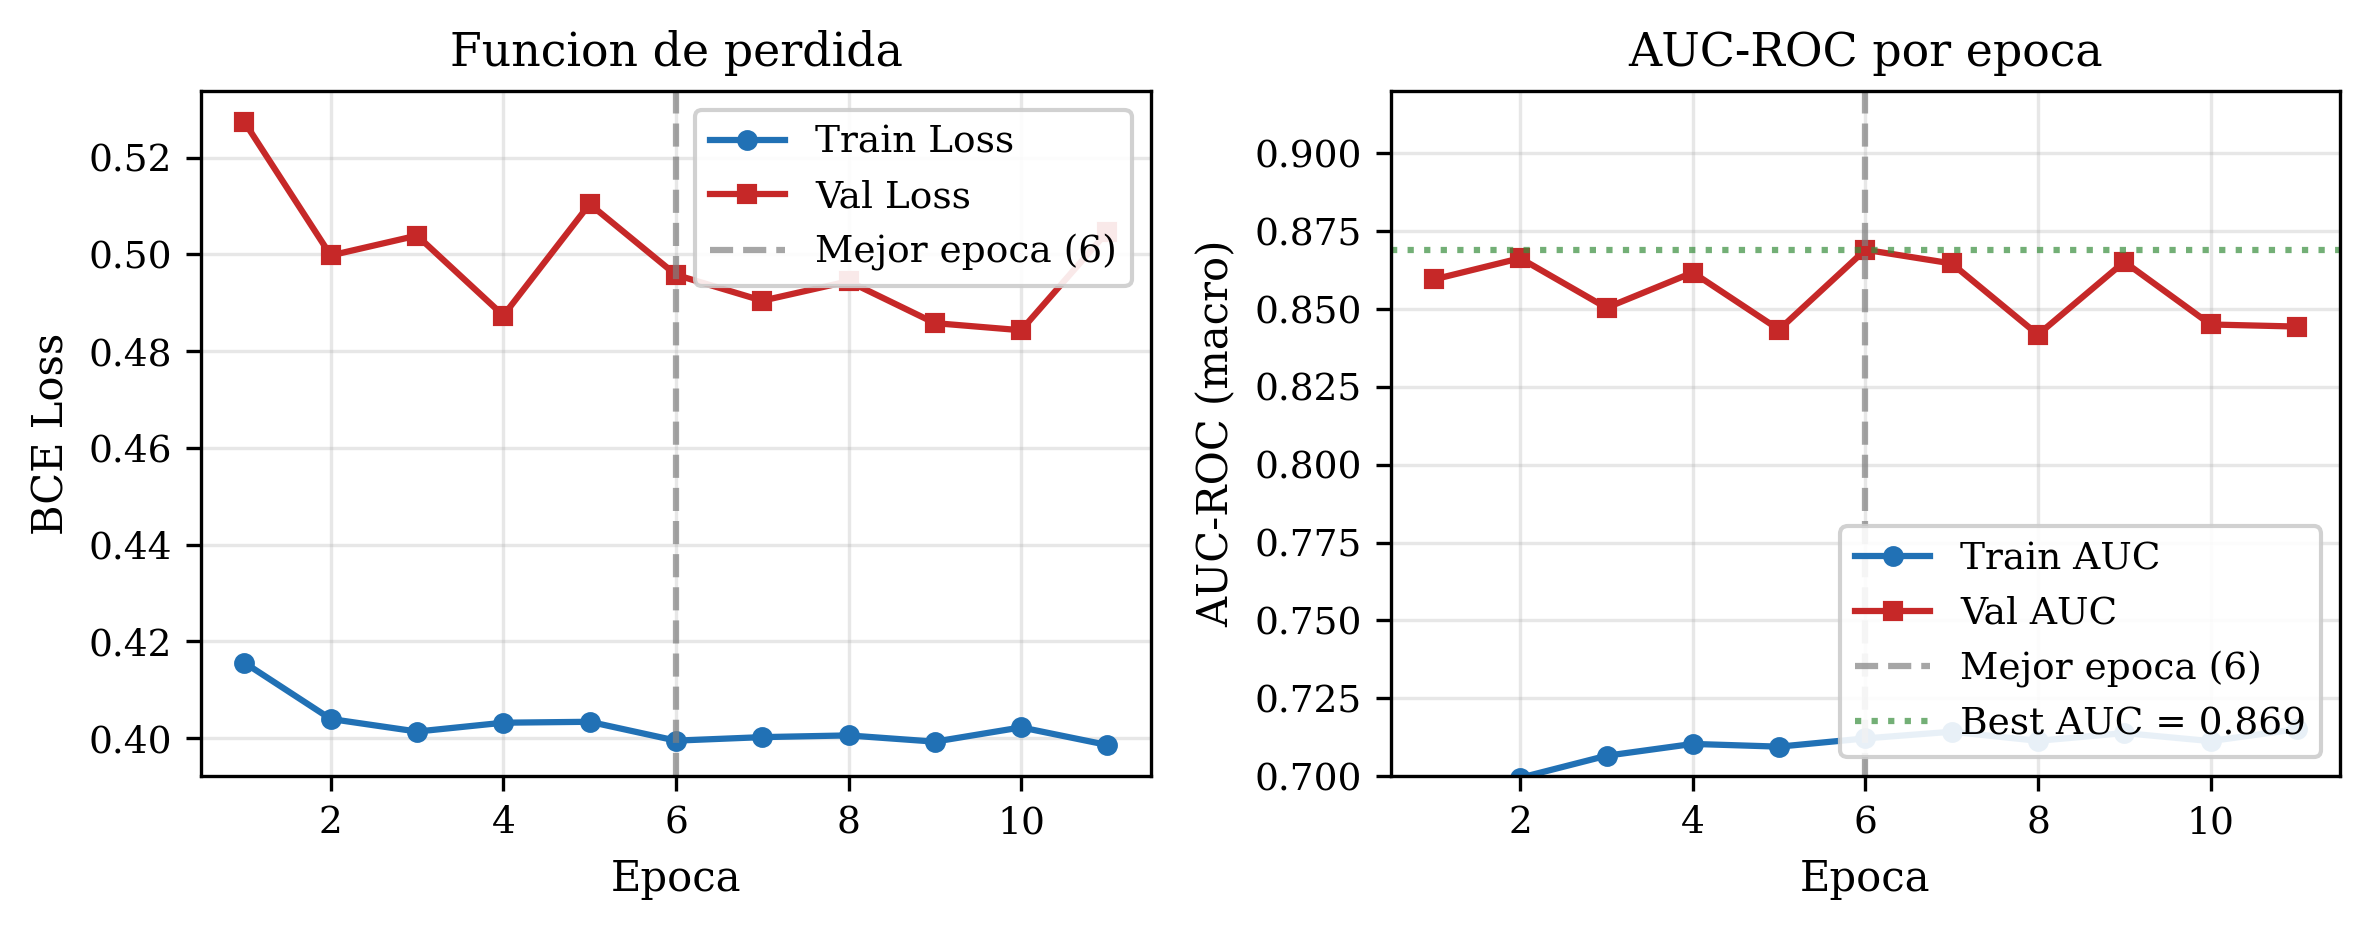
\includegraphics[width=0.85\textwidth]{figures/training-curves.png}
    \caption{Curvas de entrenamiento del modelo original: loss y AUC por \'epoca. Early Stopping activado en \'epoca 11; mejor modelo restaurado de \'epoca 6.}
    \label{fig:training}
\end{figure}

\subsection{Motivaci\'on: del notebook a producci\'on}

Existe una brecha significativa entre desarrollar un modelo de Machine Learning en un notebook y desplegarlo como servicio confiable \cite{sculley2015technical}. Los principales desaf\'ios incluyen:

\begin{itemize}
    \item \textbf{Reproducibilidad}: el modelo debe comportarse id\'enticamente en cualquier m\'aquina.
    \item \textbf{Aislamiento}: las dependencias del modelo no deben interferir con el sistema host.
    \item \textbf{Escalabilidad}: el servicio debe poder desplegarse en cualquier infraestructura cloud.
    \item \textbf{Confiabilidad}: cada cambio debe pasar por validaciones autom\'aticas antes de producción.
\end{itemize}

La containerizaci\'on con Docker y los pipelines de CI/CD resuelven estos desaf\'ios de forma est\'andar en la industria \cite{gift2021mlops}.

\subsection{Objetivo}

Empaquetar el modelo Chest Xpert AI como un servicio HTTP containerizado que:
\begin{enumerate}
    \item Arranque con un solo comando (\texttt{docker run}).
    \item Reciba una radiograf\'ia de t\'orax y devuelva predicciones de cinco patolog\'ias.
    \item Aplique las mejores pr\'acticas de Docker, CI/CD y MLOps vigentes en 2026.
    \item Se publique autom\'aticamente en un registry p\'ublico (GHCR).
\end{enumerate}

\begin{figure}[H]
    \centering
    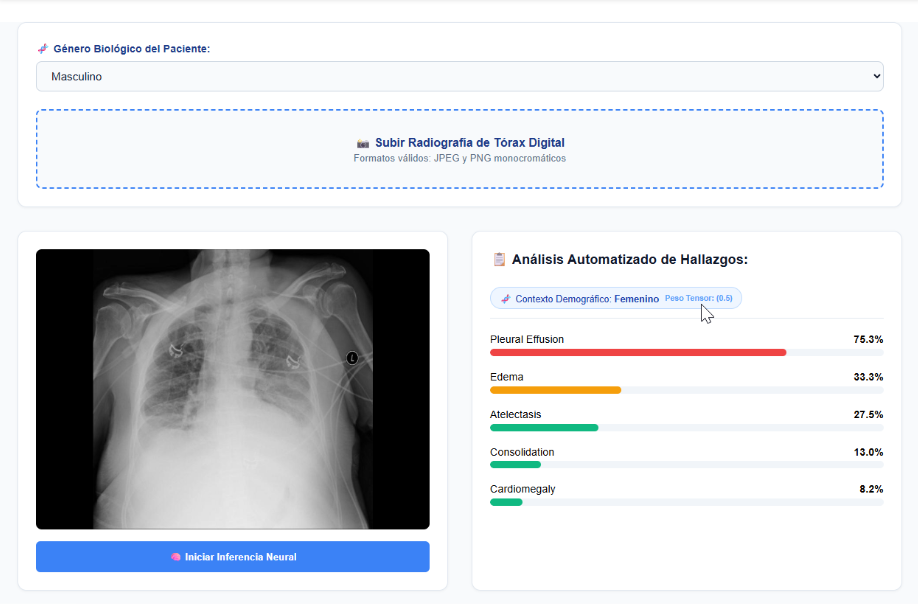
\includegraphics[width=0.85\textwidth]{figures/fullstack-plus-model-application.png}
    \caption{Arquitectura general del ecosistema Chest Xpert AI: modelo de entrenamiento, backend (FastAPI + ONNX), y frontend (Angular).}
    \label{fig:fullstack}
\end{figure}
